\section{Formal Analysis using Alloy}
In the alloy model, in order to be safer w.r.t. the requirements that have been stated in this document, critical aspects have been modeled. 
In particular, the following vital goals have been asserted:
\begin{enumerate}
\item[{[G3]}] Once the health parameters of a user have been observed below the threshold for the first time after one hour, an ambulance is sent to the user location
\item[{[G12]}]  Allow a third party to access data specified in a request if the user accepts the request or if he accepted one or more requests from the same third party that provided access to the same data 
\item[{[G13]}] Allow a third party to access statistical and anonymized data if and only if the number of individual involved is greater than 1000. This is satisfied as soon as the request is approved  
\end{enumerate}

Note on the alloy model: 
\begin{itemize}
\item Some trivial domain assumptions are written in order to prove the goals. 
However, they are not stated in the domain assumption chapter of this document 
\item The context of G3 has been modeled considering that a user uses the AutomatedSOS service at most once in an hour. 
This allows to prove the goals, without loss of generality 
\item For G13, the fact that the aggregated request is satisfied as soon as it is approved, has not been proven: the part considered critical is the access to the demanded information 
\item The constraint on the number of people involved in an aggregated request is modified without loss of generality: the group dimension has to be greater than 5 
\end{itemize}

\lstinputlisting[language=alloy]{Alloy/trackme.als}

To give a better understanding of the world environment, the following images are shown:
\begin{itemize}
\item Data4Help world: it defines better how the world of the service Data4Help works
\begin{figure}[H]
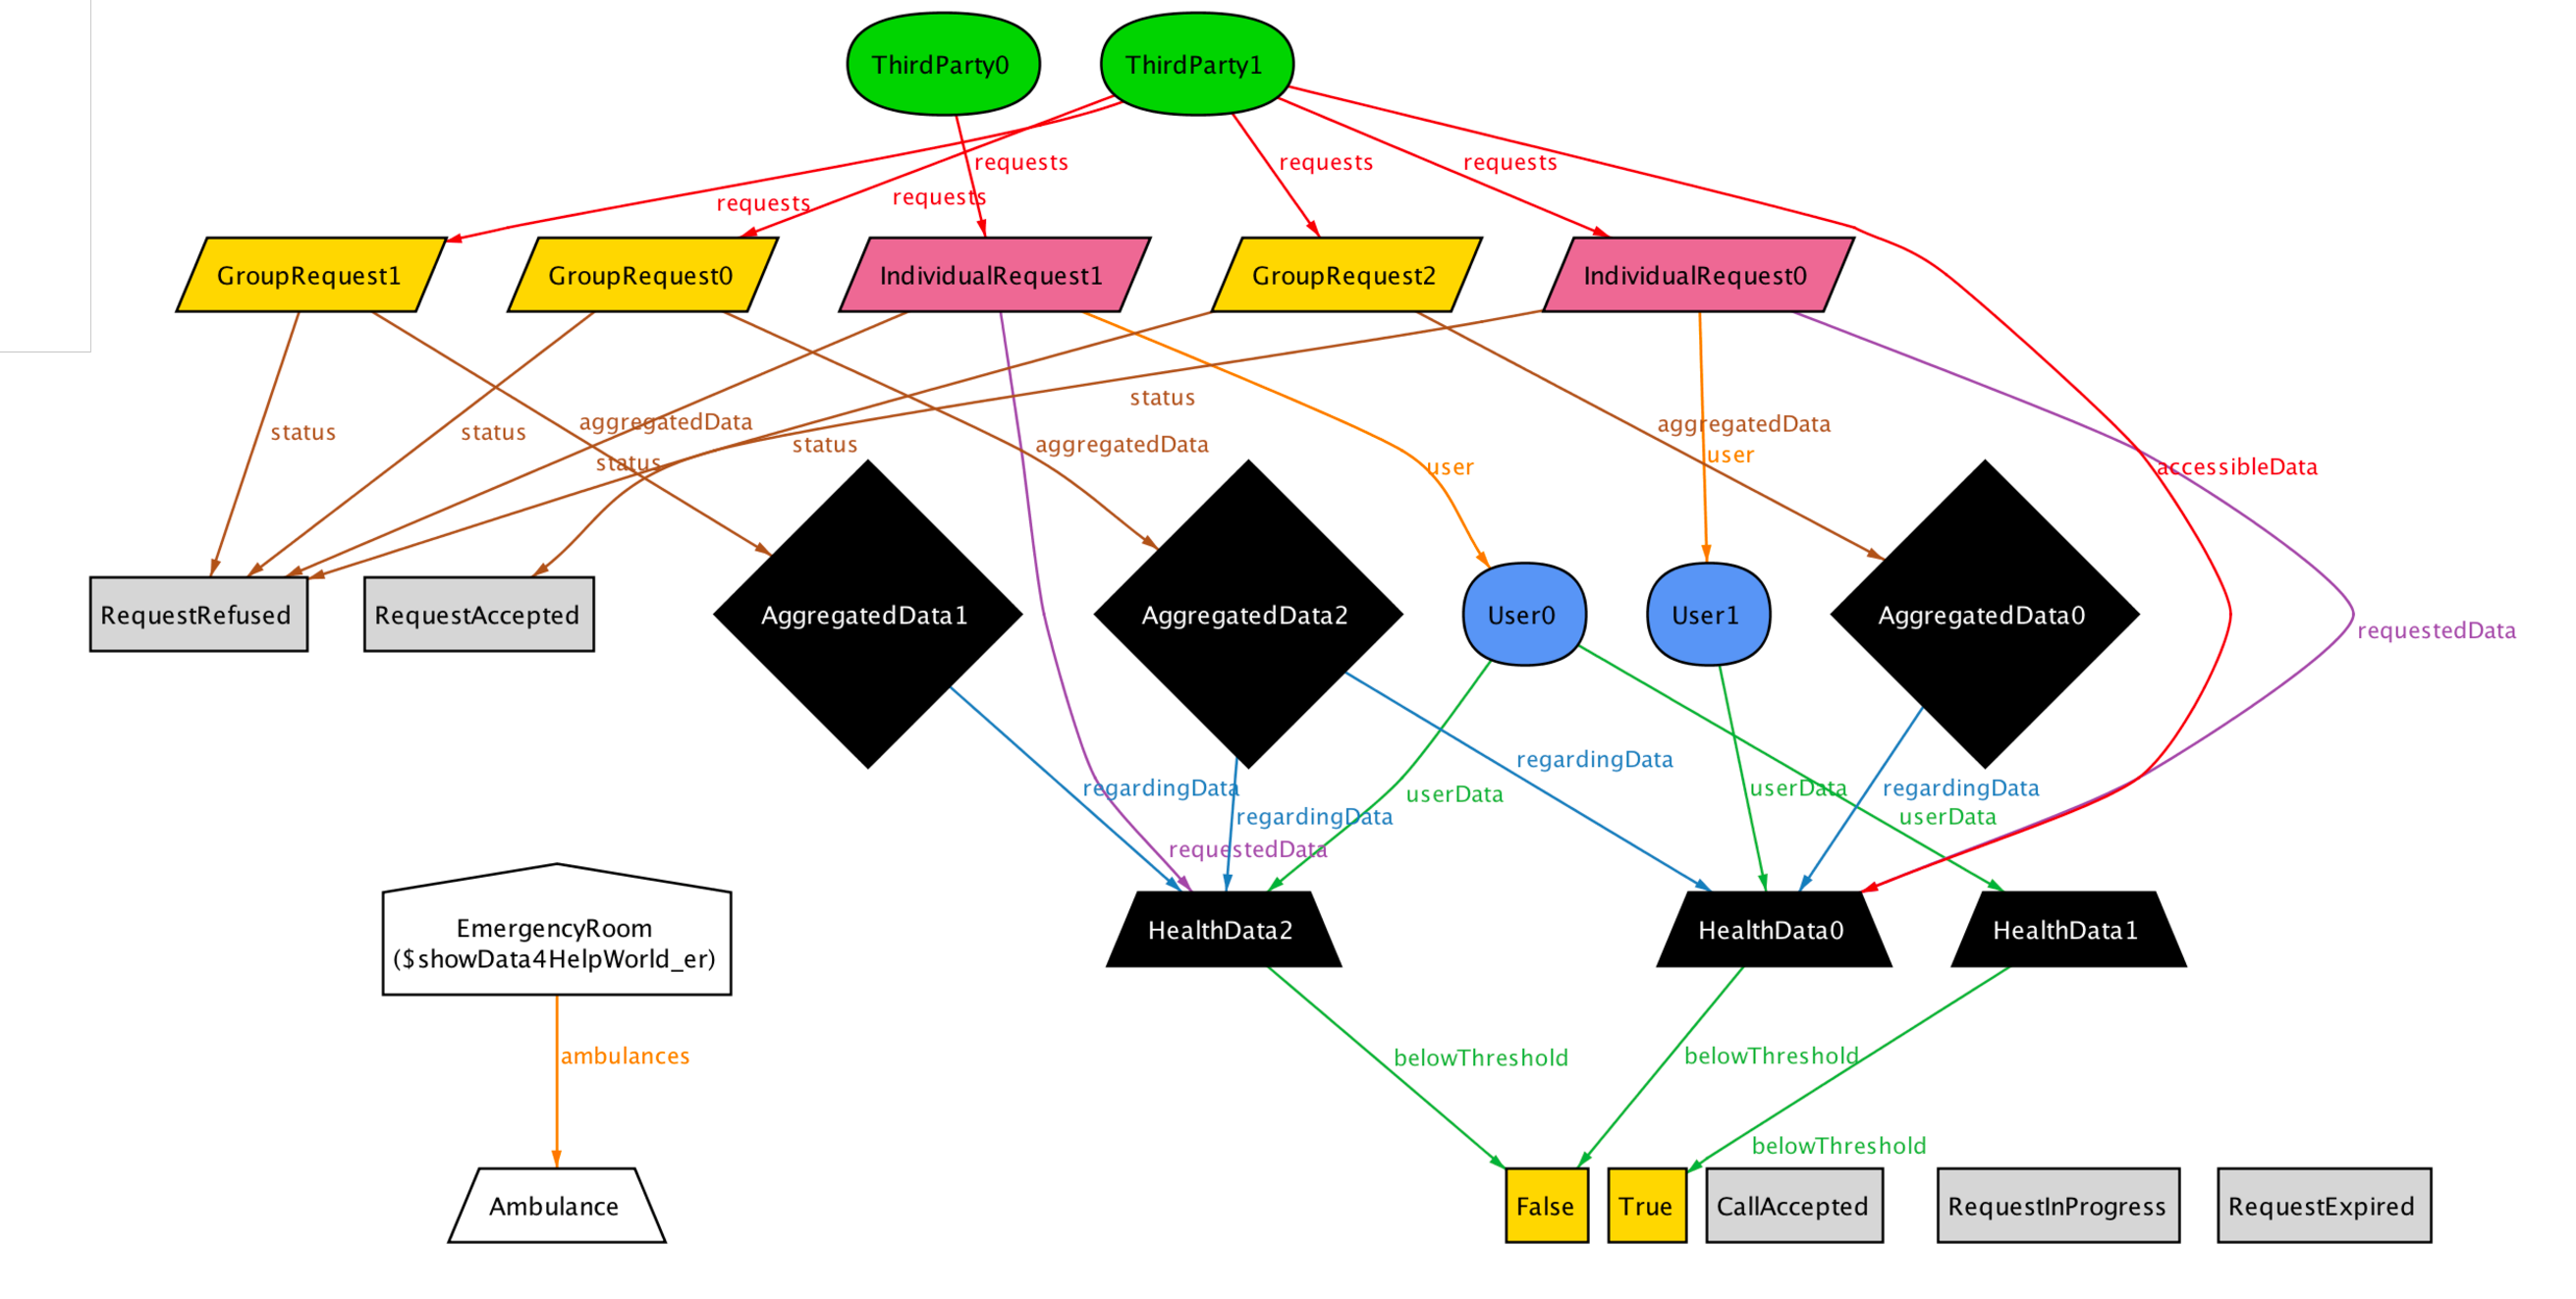
\includegraphics[width=\linewidth]{Images/world1}
\caption{ Data4Help World }
\label{fig:world1}
\end{figure}

\item AutomatedSOS world: it defines better how the world of the service AutomatedSOS works
\begin{figure}[H]
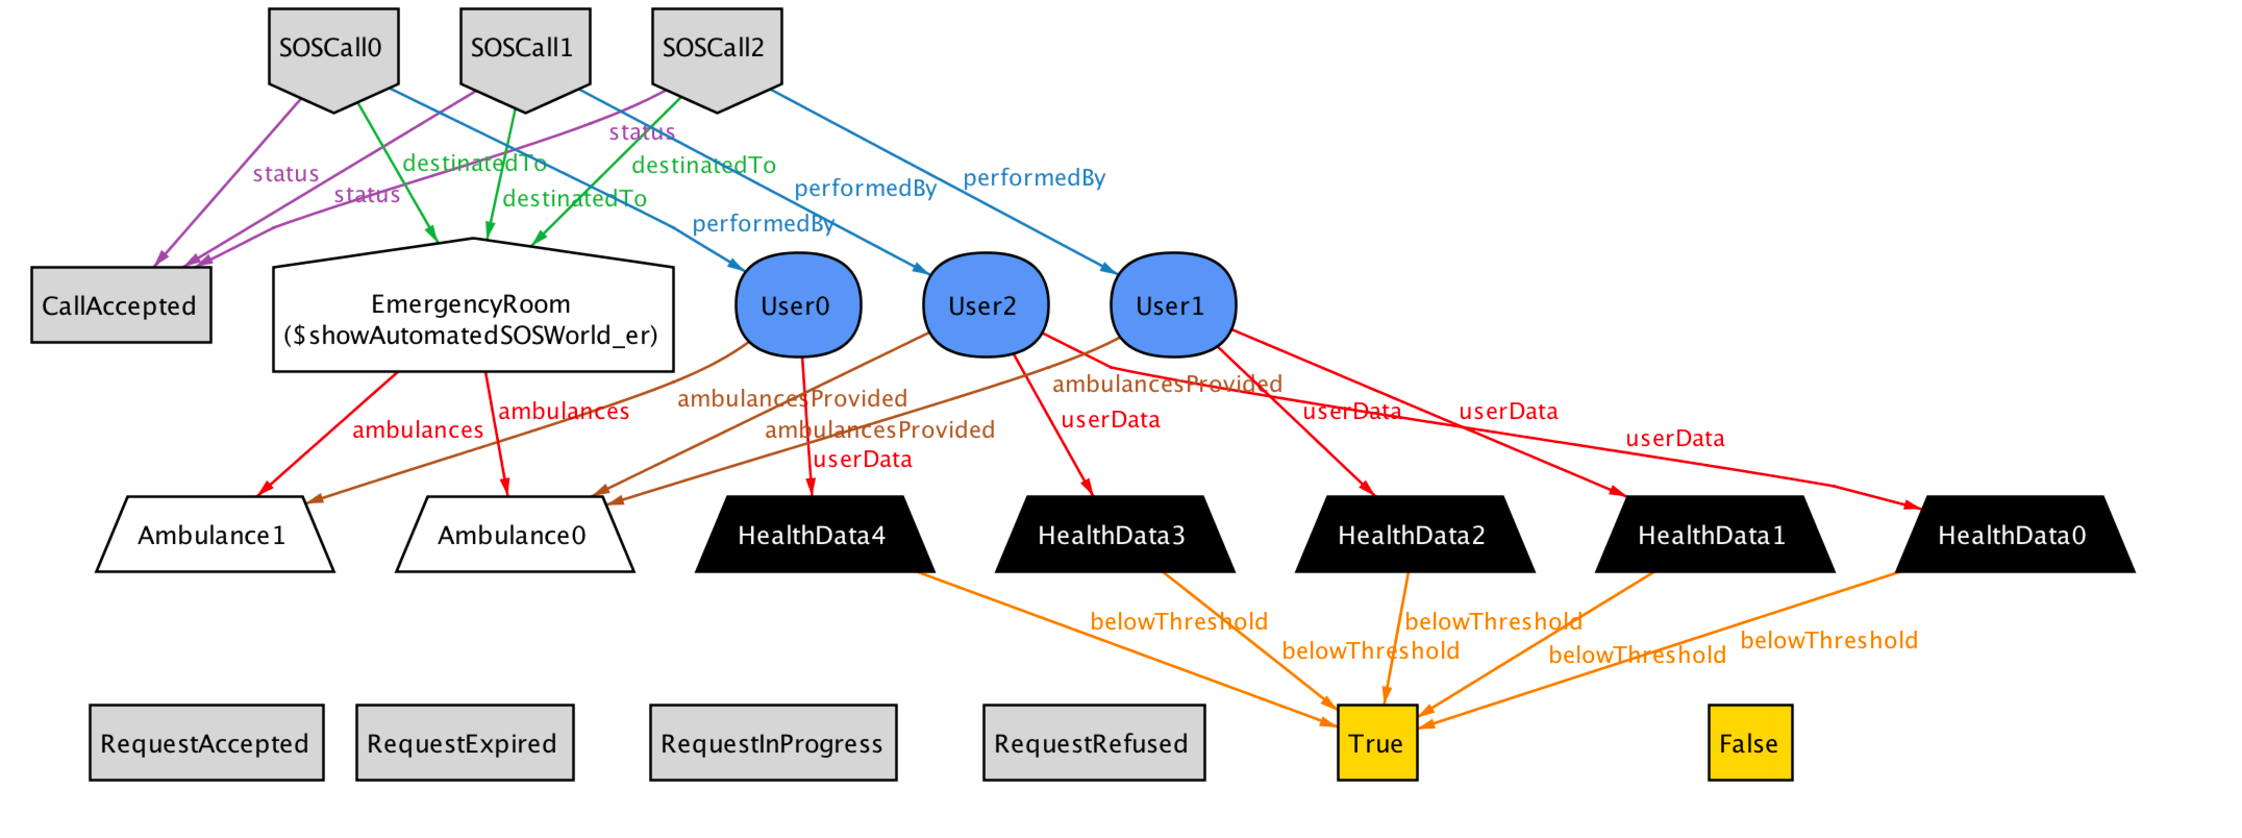
\includegraphics[width=\linewidth]{Images/world2}
\caption{ AutomatedSOS World }
\label{fig:world2}
\end{figure}
 

\end{itemize}
\subsection{Alloy results}
These are the results of the alloy model.

\begin{center}
\centering
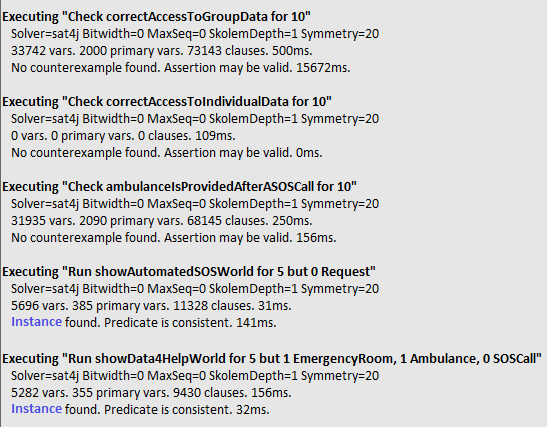
\includegraphics[width=1\textwidth]{Images/alloyResults}
\captionof{figure}{Alloy results}
\end{center}